\documentclass{article}
\usepackage{graphicx} % Required for inserting images
\usepackage{float}
\usepackage[T1]{fontenc}
\usepackage{amsmath}
\usepackage[margin=1in]{geometry}
\usepackage{booktabs}
\usepackage{tabularx}
\usepackage[hidelinks]{hyperref}

\title{Stressing the put book at 1.5x IV instead of a 60\% floor}
\author{Experiment report \textperiodcentered{} L/S Gamma Desk, QUANTT}
\date{2026-11-02}

\begin{document}

\maketitle

\textbf{Question:} On the 35\% stress-sized \texttt{hedged} put book, does sizing each entry for a one-day 20\% SPY drop with IV at max(60\%, 1.5 \ensuremath{\times} the put's IV), instead of max(60\%, the put's IV), give a higher Sharpe ratio over the full window and in each half, and a less severe maximum drawdown, at 1x and 2x spreads?

\textbf{Method:}

\begin{itemize}

\item \textbf{Pre-registration:} the hypothesis card was committed before any run (commit af47198). The research switch \texttt{stress\_\allowbreak{}vol\_\allowbreak{}mult} was committed before it, in a2d5334.

\item \textbf{Data:} the live paper rules (\texttt{configs/\allowbreak{}paper.\allowbreak{}toml}) are replayed on R2 replay snapshots v1 (config\_hash b040760187f0) over the development window 2014-06-02 to 2024-12-31. The hold-out (2025-01-01 to 2026-07-10) was not used.

\item \textbf{Book:} every variant is the \texttt{hedged} book of 2026-10-22-stress-sized-puts.

\begin{itemize}

\item An always-on short 25-delta put, with the signal ignored and the flat exit off.

\item Sized at each entry to the most contracts whose loss in a one-day 20\% SPY drop stays within the budget, counting the hedge gain and the 10-share band gap.

\item Hedged daily with a 10-share band. Stop at 1x the credit, profit-take at 50\% and time exit at 7 DTE.

\end{itemize}

\item \textbf{Variants:}

\begin{itemize}

\item \texttt{shock15} (primary): stress IV max(60\%, 1.5 \ensuremath{\times} IV), budget 35\%;

\item \texttt{budget25}: budget 25\%, today's shock max(60\%, IV);

\item \texttt{budget15}: budget 15\%, today's shock.

\end{itemize}

\item \textbf{Comparison:} the registered \texttt{2026-\allowbreak{}10-\allowbreak{}22-\allowbreak{}stress-\allowbreak{}sized-\allowbreak{}puts/\allowbreak{}hedged} runs at the same spread multiple, reused and not rerun. With the new switch off, the engine reproduces that book's equity exactly.

\item \textbf{Costs and schedule:} every variant was run at 1x and 2x spreads. \$0.65 per contract and \$0.005 per share, with a \$1 minimum per order. Decisions, exits and hedges run once a day at 10:15 ET.

\end{itemize}

\section{Result vs the pass bar}

Every check had to hold at 1x and 2x. The Sharpe ratio is annualised from daily net P\&L. Maximum drawdown is the largest fall in cumulative net P\&L from a previous peak, in USD.

\begin{center}\small
\begin{tabularx}{\linewidth}{>{\raggedright\arraybackslash}X l l l l >{\raggedright\arraybackslash}X}
\toprule
\textbf{Check (\texttt{shock15} vs \texttt{hedged})} & \textbf{1x value} & \textbf{1x bar} & \textbf{2x value} & \textbf{2x bar} & \textbf{Result} \\
\midrule
Sharpe, full window & 0.51 & > 0.52 & 0.40 & > 0.43 & \textbf{fail} \\
Sharpe, 2014-06 to 2019-12 & 0.84 & > 0.84 & 0.72 & > 0.72 & \textbf{fail (tie)} \\
Sharpe, 2020-01 to 2024-12 & 0.39 & > 0.48 & 0.27 & > 0.38 & \textbf{fail} \\
Max drawdown less severe & \$60,228 & < \$70,362 & \$65,032 & < \$75,488 & pass \\
Event floor: entries with IV > 40\% & 4 & \ensuremath{\geq} 3 &  &  & met \\
\bottomrule
\end{tabularx}
\end{center}

\textbf{Verdict: failed.} The 1.5x shock cut the drawdown by about \$10k, but it cost \$28.5k of net P\&L at 1x (\$27.8k at 2x), and the Sharpe ratio fell over the full window and in 2020-2024. The book still makes money: \$93.0k at 1x and \$73.3k at 2x.

\subsection{Full-window numbers (not part of the bar)}

\begin{center}\small
\begin{tabularx}{\linewidth}{>{\raggedright\arraybackslash}X l l l >{\raggedright\arraybackslash}X >{\raggedright\arraybackslash}X l >{\raggedright\arraybackslash}X}
\toprule
\textbf{Book} & \textbf{Net P\&L} & \textbf{Sharpe} & \textbf{Max drawdown} & \textbf{P\&L /\allowbreak{} drawdown} & \textbf{ES 5\% (daily)} & \textbf{Round trips} & \textbf{Commissions (options /\allowbreak{} hedges)} \\
\midrule
\texttt{hedged} 1x & \$121,482 & 0.52 & \$70,362 & 1.73 & \ensuremath{-}\$3,016 & 182 & \$5,955 /\allowbreak{} \$2,868 \\
\texttt{shock15} 1x & \$92,985 & 0.51 & \$60,228 & 1.54 & \ensuremath{-}\$2,826 & 182 & \$5,862 /\allowbreak{} \$2,842 \\
\texttt{budget25} 1x & \$80,340 & 0.48 & \$55,102 & 1.46 & \ensuremath{-}\$2,135 & 184 & \$4,264 /\allowbreak{} \$2,494 \\
\texttt{budget15} 1x & \$49,858 & 0.51 & \$29,302 & 1.70 & \ensuremath{-}\$1,234 & 181 & \$2,452 /\allowbreak{} \$2,123 \\
\texttt{hedged} 2x & \$101,172 & 0.43 & \$75,488 & 1.34 & \ensuremath{-}\$3,094 & 181 & \$5,918 /\allowbreak{} \$2,863 \\
\texttt{shock15} 2x & \$73,349 & 0.40 & \$65,032 & 1.13 & \ensuremath{-}\$2,905 & 181 & \$5,824 /\allowbreak{} \$2,837 \\
\texttt{budget25} 2x & \$72,339 & 0.43 & \$53,701 & 1.35 & \ensuremath{-}\$2,156 & 181 & \$4,186 /\allowbreak{} \$2,498 \\
\texttt{budget15} 2x & \$41,938 & 0.43 & \$31,427 & 1.33 & \ensuremath{-}\$1,260 & 180 & \$2,434 /\allowbreak{} \$2,118 \\
\bottomrule
\end{tabularx}
\end{center}

\section{Charts}

\begin{figure}[H]\centering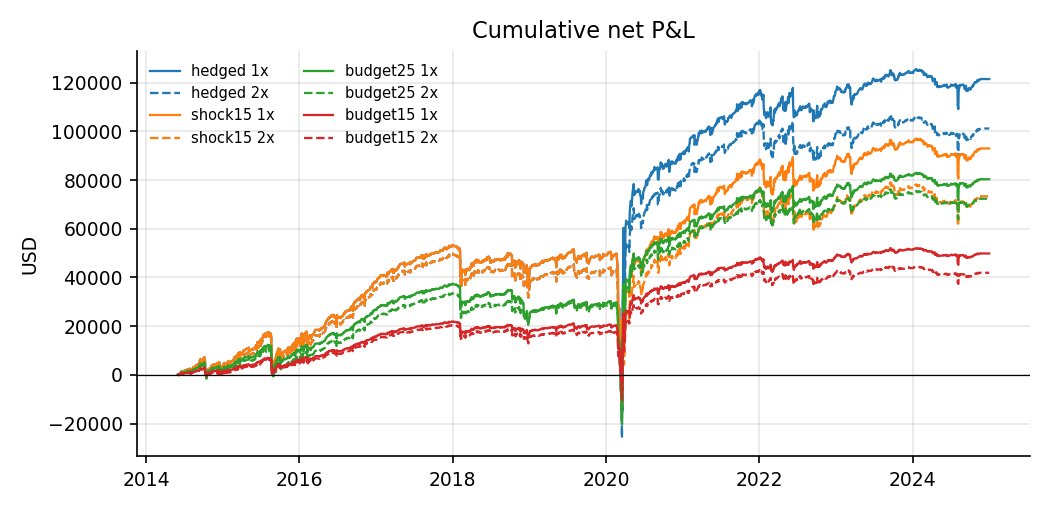
\includegraphics[width=0.92\linewidth]{figures/cum_pnl.png}\caption{Cumulative net P\&L, 1x solid and 2x dashed}\end{figure}

\texttt{shock15} tracks \texttt{hedged} exactly until March 2020, then ends about \$28k lower. The two budget books are scaled-down versions of \texttt{hedged} all the way through.

\begin{figure}[H]\centering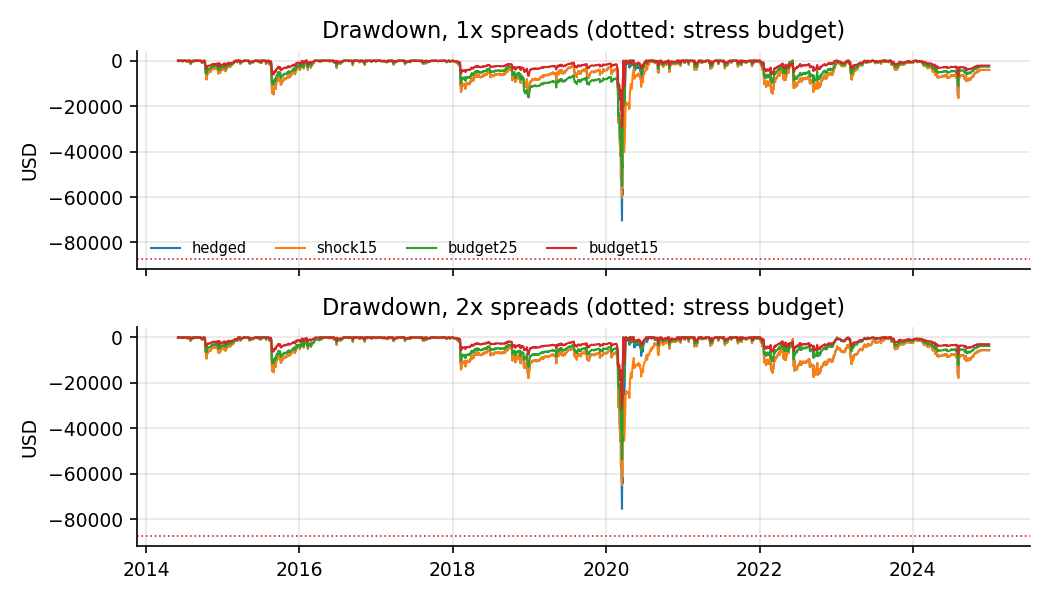
\includegraphics[width=0.92\linewidth]{figures/drawdown.png}\caption{Drawdown at 1x and 2x spreads}\end{figure}

Every book's worst drawdown runs from the January 2018 peak to the 17 March 2020 trough. The 1.5x shock makes that trough about \$10k shallower. The 25\% and 15\% budgets make it \$15k and \$41k shallower at 1x.

\begin{figure}[H]\centering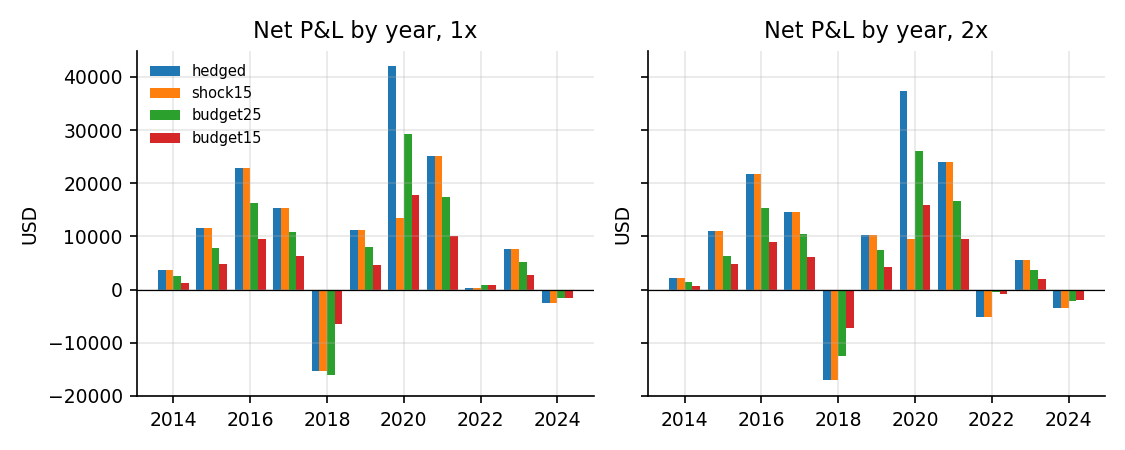
\includegraphics[width=0.92\linewidth]{figures/yearly.png}\caption{Net P\&L by year}\end{figure}

\texttt{shock15} matches \texttt{hedged} in every year except 2020, where it made \$13.5k against \$42.0k at 1x. The budget books earn about 70\% (25\%) and 40\% (15\%) of \texttt{hedged} in most years.

\begin{figure}[H]\centering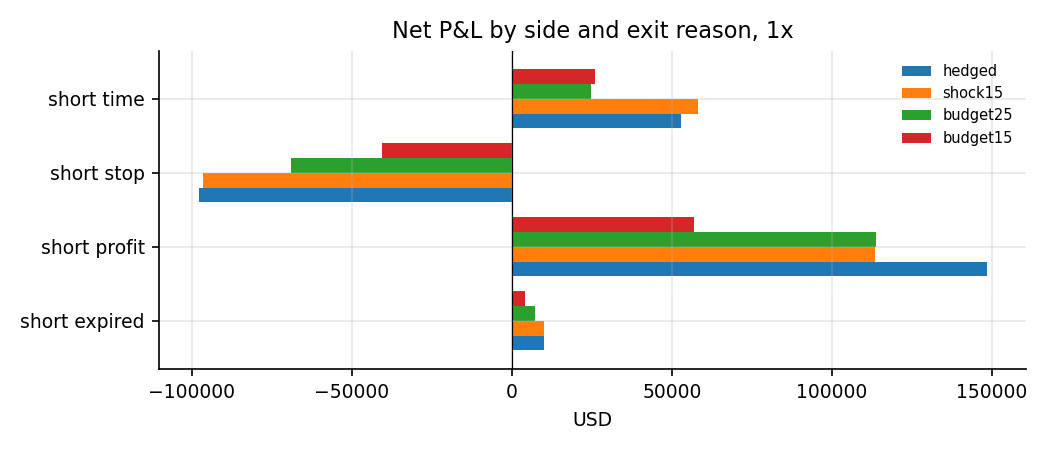
\includegraphics[width=0.92\linewidth]{figures/by_reason.png}\caption{Net P\&L by side and exit reason, 1x}\end{figure}

The shock mostly removed profit-take P\&L: the 13 March 2020 put closed at its 50\% profit-take with half as many contracts.

\begin{figure}[H]\centering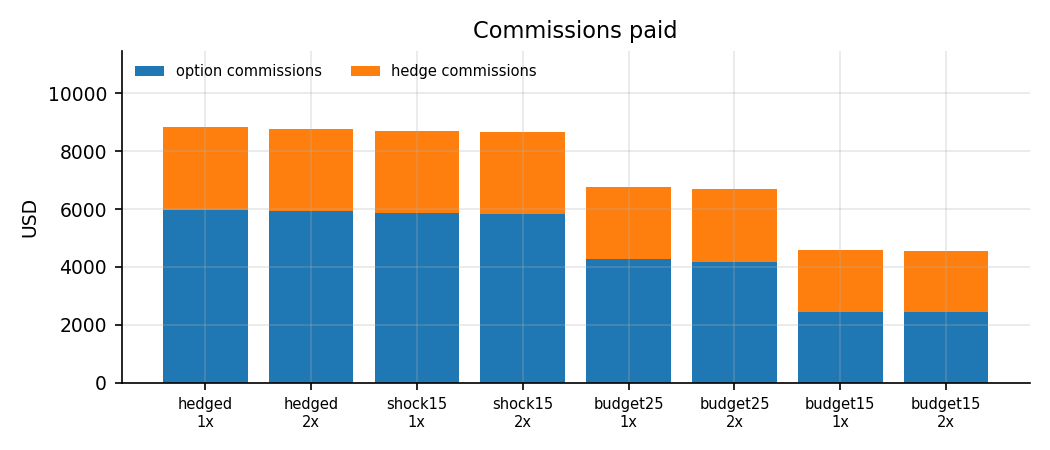
\includegraphics[width=0.92\linewidth]{figures/fees.png}\caption{Commissions paid}\end{figure}

Commissions barely move under the shock, because only 4 entries changed size. The smaller budgets save about \$2k and \$4k at 1x.

\begin{figure}[H]\centering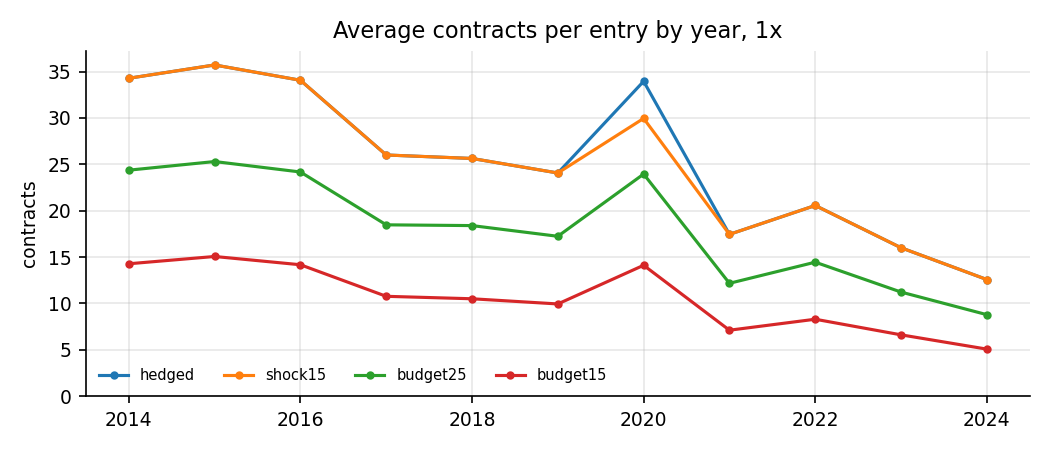
\includegraphics[width=0.92\linewidth]{figures/contracts.png}\caption{Average contracts per entry by year, 1x}\end{figure}

The shock only changes 2020. The budget books sell about 70\% and 40\% as many contracts as \texttt{hedged} every year.

\begin{figure}[H]\centering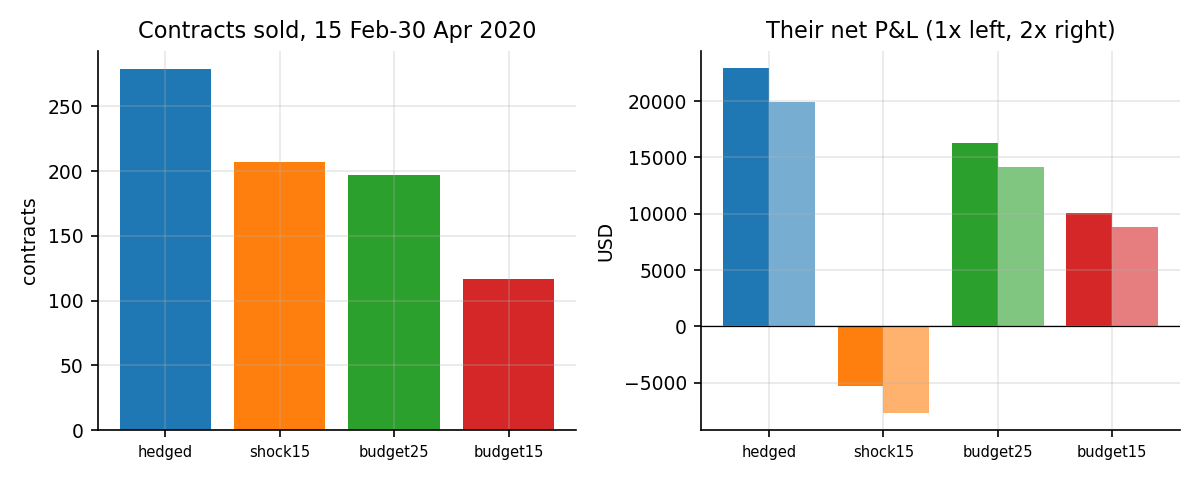
\includegraphics[width=0.92\linewidth]{figures/march2020.png}\caption{Contracts sold and net P\&L of round trips opened 15 February to 30 April 2020}\end{figure}

In the crash window, \texttt{shock15} sold 207 contracts against 279. Those round trips lost \$5.3k, against a \$22.9k profit for \texttt{hedged}. The 25\% budget sold even fewer contracts (197) and still made \$16.3k.

\section{Analysis}

\textbf{The shock changed four trades, all in 2020.} Before 2020, no entry had a put IV above 40\% (the level where 1.5 \ensuremath{\times} IV exceeds the 60\% floor), so \texttt{shock15} is identical to \texttt{hedged} from 2014 to 2019. All 182 round trips open at the same times in both books; 178 have the same size. The four that changed were the 2 March, 13 March, 24 March and 17 April 2020 entries, and every difference in P\&L comes from them. The pre-registered 2014-2019 Sharpe check therefore could only tie. That is a design flaw in the bar, but it doesn't decide the verdict: the full-window and 2020-2024 checks fail too.

\textbf{The shock mostly cut the winning trade.} The two stop-outs in the crash came from puts sold on 26 February and 2 March, before IV had risen much (the 2 March put's IV was about 42\%). The shock left the first unchanged at 27 contracts and trimmed the second from 41 to 39. The stops on those two still cost \$48k. The 13 March put was sold at an IV near 68\%, so the shock cut it from 100 to 51 contracts. That put made \$70.7k in \texttt{hedged} and \$36.1k here. The 24 March put went from 71 to 51 contracts and lost \$4.2k instead of \$9.4k. Net, the four changed trades gave up \$28.3k at 1x. A shock that scales with IV binds hardest after the crash has started, when puts were most profitable to sell in this sample. It does nothing about the first leg of a crash, which starts from moderate IV. This is one episode, so it shows the mechanism, not a reliable estimate of its size.

\textbf{Smaller fixed budgets don't improve the risk-adjusted return either.} \texttt{budget25} and \texttt{budget15} scale every entry to about 70\% and 40\% of the \texttt{hedged} size (rounded down to whole contracts). Their full-window Sharpe ratios are 0.48 and 0.51 at 1x and 0.43 and 0.43 at 2x, against 0.52 and 0.43. P\&L per dollar of drawdown is similar or lower (1.46 to 1.70 against 1.73 at 1x; 1.33-1.35 against 1.34 at 2x). So a smaller budget gives a smaller version of the same book. It doesn't improve risk-adjusted returns. The 25\% book's 2014-2019 Sharpe (0.69 against 0.84) is lower, partly because of path changes in 2018: 7 of its 184 round trips open at different times from \texttt{hedged}, and it lost slightly more that year. This suggests the 2026-11-02 slope-sizing result (Sharpe 0.64) is not just the effect of a smaller budget.

\section{Verdict}

\textbf{Failed} on the pre-registered bar at 1x and 2x: Sharpe fell over the full window and in 2020-2024 (and tied in 2014-2019), although the drawdown was smaller. Archive the 1.5x IV shock. The sizing choice between 35\%, 25\% and 15\% is a risk-appetite decision for the PM: on this sample, all three budgets have about the same Sharpe, and drawdown scales with the budget. Neither variant changes what the 2026-10-22 hold-out would test. If the desk wants protection for the first leg of a crash, a size cap based on the drop already taken (or a calendar or notional cap) would need its own card.

\section{Caveats}

\begin{itemize}

\item \textbf{In-sample:} the idea comes from the 2026-10-22 results on this same window, and the book was chosen after those results. Before pre-registration, the desk saw that the reference had 4 entries with IV above 40\%, but not their dates or P\&L.

\item \textbf{One episode:} every difference between \texttt{shock15} and \texttt{hedged} comes from 4 entries in March-April 2020.

\item \textbf{Bar design:} the 2014-2019 Sharpe check could not be met, because the shock never binds before 2020.

\item \textbf{Spread model:} fitted on about two weeks of calm 2026 live quotes. Large March 2020 fills (40-100 contracts) use the one-contract spread model; the 2x run is the stress test.

\item \textbf{Data gaps:} R2 has no month-end weekdays, so about 3.3\% of scheduled times are skipped.

\item \textbf{Model limits:} a Black-Scholes stress loss with flat IV across strikes; margin is not modelled. Spot comes from put-call parity on a 30-minute grid from 10:15 to 15:45.

\end{itemize}

\section{Trials}

6 trials for this experiment (3 variants \ensuremath{\times} 1x and 2x, one run of \texttt{experiment.\allowbreak{}py}), plus the baseline's 2. The \texttt{hedged} reference was reused, not rerun. All six rows are tagged \texttt{-\allowbreak{}dirty}, at commits 79b09a1 (\texttt{shock15} 1x) and 3568520 (the rest). Both commits contain this card's pre-registration (af47198), and HEAD moved during the run because other cards in the same batch were being pre-registered. The engine, \texttt{backtest.\allowbreak{}toml} and this card's config and script were unchanged between af47198 and 3568520. The dirty files were other cards' uncommitted files in the shared working tree. Two charts were fixed afterwards in this card's script (drawdown legend position, a clipped title) and rebuilt with \texttt{-\allowbreak{}-\allowbreak{}report-\allowbreak{}only}, which adds no trials. The pass bar was not changed.

\end{document}
